\documentclass[11pt,letterpaper]{article}
\usepackage[T1]{fontenc}
\usepackage{lmodern,amsmath,amssymb,amsthm,mathtools}
\usepackage[margin=0.9in]{geometry}
\usepackage{microtype,booktabs,longtable,array,graphicx,enumitem,xurl,needspace}
\usepackage[dvipsnames]{xcolor}
\usepackage{fancyhdr}
\usepackage[colorlinks=true,linkcolor=MidnightBlue,citecolor=MidnightBlue,urlcolor=MidnightBlue]{hyperref}
\hypersetup{pdftitle={Selective coefficient extraction for explicit ZFC consistency equations},pdfauthor={Research report prepared for Vladimir Reshetnikov's ProveIt project}}
\setlength{\headheight}{14pt}
\pagestyle{fancy}\fancyhf{}\fancyhead[L]{\small Selective Diophantine consistency equations}\fancyhead[R]{\small 23 October 2026}\fancyfoot[C]{\thepage}
\setlength{\parskip}{4pt}\setlength{\parindent}{0pt}
\setlist{topsep=4pt,itemsep=3pt,parsep=0pt}
\allowdisplaybreaks
\newtheorem{theorem}{Theorem}[section]
\newtheorem{lemma}[theorem]{Lemma}
\newtheorem{proposition}[theorem]{Proposition}
\newtheorem{corollary}[theorem]{Corollary}
\theoremstyle{definition}\newtheorem{definition}[theorem]{Definition}
\newcommand{\Z}{\mathbb Z}\newcommand{\N}{\mathbb N}\newcommand{\Pos}{\mathbb Z_{>0}}
\newcommand{\Con}{\operatorname{Con}}\newcommand{\pc}{\operatorname{pc}}
\newcommand{\BB}{\mathcal B}\newcommand{\Dc}{\mathcal D}\newcommand{\Ccap}{\mathcal C}
\newcommand{\coef}{\operatorname{coeff}}\newcommand{\Sq}{\operatorname{Sq}}
\newcommand{\file}[1]{{\small\nolinkurl{#1}}}

\begin{document}
\hypersetup{pageanchor=false}
\begin{titlepage}
\vspace*{0.6in}
{\large\color{MidnightBlue} PROVEIT RESEARCH REPORT\par}
\vspace{0.35in}
{\Huge\bfseries Selective coefficient extraction\par}
\vspace{0.12in}
{\LARGE for explicit ZFC consistency equations\par}
\vspace{0.45in}
{\large A smaller polynomial in ten unrestricted integers,\par
and a companion polynomial in nine positive integers\par}
\vspace{0.55in}
\begin{center}
\renewcommand{\arraystretch}{1.35}
\begin{tabular}{lrr}
\toprule
Witness domain & Exact degree & Binary operations\\
\midrule
$\Z^{10}$ & $35\,876\,184$ & $640$\\
$\Pos^9$ & $19\,615\,180$ & $606$\\
$\N^9$, with $0\in\N$ & $19\,615\,180$ & $609$\\
\bottomrule
\end{tabular}
\end{center}
\vspace{0.45in}
Prepared for Vladimir Reshetnikov's ProveIt project.\\
23 October 2026.\\[6pt]
Repository snapshot:\\
\texttt{124c07c0b77a9e20e84676514d8b1ff78536ea3f}.
\vfill
\textbf{Evidence level.} Explicit coefficient data, complete finite arithmetic
circuits, ordinary mathematical proofs of the new reductions, and independent
finite audits. The unbounded compiler and number-theoretic theorems are named
dependencies. This report does not claim a new end-to-end proof-assistant
certificate or a global simplicity minimum.
\end{titlepage}
\hypersetup{pageanchor=true}

\begin{abstract}
We construct an explicit integer-coefficient polynomial in ten unrestricted
integer variables whose lack of solutions is equivalent, by an arithmetic
argument formalizable in ZFC, to syntactic consistency of ZFC. Its exact total
degree is $35\,876\,184$ and a literal division-free evaluator has 640 binary
operations. Relative to the current package-40 ten-integer construction at
the reviewed repository snapshot, the degree is smaller by a factor of 6.62
and the evaluator has 142 fewer operations. A companion Jones construction
uses nine positive variables, degree $19\,615\,180$, and 606 operations.

The improvement comes from changing the coefficient-extraction problem.
The source contains 22 quadratic equations in 31 positive variables, but
only 62 of the 528 possible padded quadratic monomials occur. Their positions
must be isolated; positions of unused monomials may collide. An explicit
weight list of span 175 suffices, instead of the inherited Sidon span 799.
Positivity is applied once to the common packed word, avoiding expansion of
every source equation. Nonuniform target positions and removal of common
padding further shorten the exponent range. Exact symbolic audits verify
every extracted quadratic equation. All coefficients are supplied by finite
recipes and authenticated binary payloads; none is chosen by an unspecified
existence principle. The work preserves the inherited compiler tuple and
attributes the nine- and ten-variable arithmetic bridges to their sources.
\end{abstract}

\setcounter{tocdepth}{1}
\tableofcontents
\newpage

\section{Results and their precise meaning}
\label{sec:results}

Let $\Con(\mathrm{ZFC})$ mean that there is no finite derivation of falsity
from the repository's fixed, effectively presented ZFC axiom predicate.
We use $\N=\{0,1,2,\ldots\}$ and distinguish positive, nonnegative, and
unrestricted integer witnesses throughout.

\begin{theorem}[Explicit consistency equations]
\label{thm:main}
The coefficient data and substitution rules in this report define fixed
polynomials $P_{10}\in\Z[f,g,h,k,l,w,x,y,z,m]$ and $P_9\in\Z[X_1,\ldots,X_9]$.
Using the pinned positive-parent compiler theorem and the arithmetic bridges
specified in Sections~\ref{sec:parent}, \ref{sec:tenproof}, and~\ref{sec:nine},
the following equivalences have proofs formalizable in ZFC:
\begin{align}
\neg\exists\mathbf x\in\Z^{10}\;P_{10}(\mathbf x)=0
 &\quad\longleftrightarrow\quad \Con(\mathrm{ZFC}),\label{eq:main10}\\
\neg\exists\mathbf x\in\Pos^9\;P_9(\mathbf x)=0
 &\quad\longleftrightarrow\quad \Con(\mathrm{ZFC}).\label{eq:main9}
\end{align}
The exact degrees are respectively $35\,876\,184$ and $19\,615\,180$.
The supplied evaluators use respectively 640 and 606 binary additions,
subtractions, and multiplications. The nine-nonnegative version has the same
degree and 609 operations.
\end{theorem}

These are unconditional equivalences: their proofs do not assume that ZFC
is consistent or inconsistent. They do not decide either side. The precise
polynomial is specified by its finite arithmetic circuit and fixed leaves;
an expanded list of millions of monomials is unnecessary. All displayed
auxiliary names denote polynomial substitutions, not additional witnesses.

The comparison is to the current repository snapshot, including newly
placed wave-6 packages 38--45. The supplied incoming directory contains its
placement ledger; those archives have already been placed in the report
collection. The active research beside the collection also contains later
checked local degree reductions. These were included in the review
\cite{snapshot,active,package40,package45}.

\begin{center}
\renewcommand{\arraystretch}{1.15}
\begin{tabular}{llrr}
\toprule
Construction & Domain & Exact degree & Operations\\
\midrule
Package 40 & $\Z^{10}$ & $237\,520\,456$ & 782\\
This report, $P_{10}$ & $\Z^{10}$ & $35\,876\,184$ & 640\\
Package 45 & $\Pos^9$ & $129\,875\,980$ & 788\\
This report, $P_9$ & $\Pos^9$ & $19\,615\,180$ & 606\\
Inherited P67 & $\Pos^{15}$ & 155 & 67\\
Checked local P75 & $\Pos^{15}$ & 68 & 75\\
Local P74, Appendix~\ref{app:p74} & $\Pos^{15}$ & 68 & 74\\
\bottomrule
\end{tabular}
\end{center}

The main ten-integer degree decreases by $84.90\%$, while operation count
decreases by $18.16\%$. The nine-positive degree decreases by $84.90\%$,
and operations by $23.10\%$. P67 remains much shorter if operation count
alone is prioritized and fifteen positive variables are acceptable. Thus
``simplest'' has no scalar answer without specifying a domain and an ordering
of variable count, degree, arithmetic size, and coefficient size. No theorem
of global optimality, and no new universal variable-count theorem, is claimed.

\Needspace{9\baselineskip}
\subsection{What is new}
Three changes compose without altering the inherited machine or compiler:
\begin{enumerate}
\item Isolate only source-supported monomials. This replaces a full Sidon
condition by a strictly weaker finite condition on 62 protected pairs.
\item Encode positive witnesses by adding a fixed word to the single common
convolution factor. This avoids 31 separate successor substitutions in all
22 equations.
\item Choose target positions using the actual supports, then translate all
targets by the maximal common amount that keeps exponents nonnegative.
\end{enumerate}
The first two changes reduce both the necessary separation problem and the
coefficient description. The third reduces degree without introducing new
unknowns. Shared Horner evaluation turns these structural savings into the
literal circuit counts above.

\section{The fixed positive quadratic parent}
\label{sec:parent}

The parent is the pinned 31-positive-variable, 22-quadratic-equation system
retained in package 31 and independently recorded by package 40
\cite{parent,package31,package40}. Its variable order is
\begin{gather*}
J,F,\alpha,z,f,h,i,o,j,s,w,\tau,\eta,\zeta,y,\gamma,\\
N,E,P,c,a,X,D,C_2,L,F_2,V,g,I,B_{\rm aux},\Delta.
\end{gather*}
The four fixed integer ports are $\beta,K_0,M_C,M_F$, and
\[
q=\beta J+1,\qquad k=\eta+\zeta,\qquad H=4a+3,\qquad C=q-F-\alpha
\]
are affine abbreviations. All 31 witnesses here are strictly positive.
The equations, in their original order, are
\begin{gather}
L=q^2-1,\qquad N=q(L+1),\qquad X=wq,\notag\\
a=E+sN,\qquad E=X(a-E),\qquad c=k(a-E)+\eta,\notag\\
P=E(c-\eta)+k,\qquad \tau^2=P(P-k)+1,\notag\\
D=X+ac+\gamma H,\qquad \Delta=a^2+H,\qquad C_2=c^2,\notag\\
D^2=\Delta C_2+1,\qquad k=jc-V+1+hE,\notag\\
jc-V=(q-F)(N-q)-CL+(M_C+qM_F)J,\notag\\
(K_0+w)C+(q-F)-z(q-1)=1,\notag\\
F_2=f^2,\qquad V=of-c,\qquad g=y^2-V^2,\notag\\
I=iC_2,\qquad B_{\rm aux}=I^2,\qquad B_{\rm aux}=\Delta(F_2-1),\notag\\
y^2-B_{\rm aux}g=1.\label{eq:parent}
\end{gather}
For numbering, read each line from left to right. Each residual $r_j$ is
left side minus right side, with the affine abbreviations expanded. Their
complete sparse forms are supplied in \file{upstream/parent_sparse.json}.
The finite auditor reconstructs the new weighted records from this data,
keeping the four ports as independent symbolic indeterminates.

\subsection{The inherited semantic theorem}
The inherited ordinary mathematical theorem says that this positive system
has a solution exactly when K215 halts on blank input, and hence exactly
when the fixed ZFC proof predicate has a refutation. Its ingredients are
the native-window/Pell compiler, the coherent coefficient calibration,
the algebraic parent reduction, and the checked K215 endpoint
\cite{parent,package31,k215,native}.

The present report does not change any of those ingredients. In particular,
the positive transport coordinate $z$ in~\eqref{eq:parent} is the old,
unshifted parent coordinate. The complete four-port tuple is inherited from
package 31, with the mask convention already shifted by $B-1$.
Mixing that tuple with components from another package would not be justified.

The active Lean research proves a nine-natural-variable existence theorem
using a classically selected polynomial, and proves local equivalences of
several explicit short circuits. It explicitly leaves the explicit native
compiler bridge and an object-language ZFC derivation open
\cite{active}. Those are valuable separate results; they are not a new
kernel certificate for the explicit polynomials constructed here.

\subsection{Concrete coefficient data}
The four native ports have the following exact bit lengths:
\begin{center}
\begin{tabular}{lrl}
\toprule
Port & Bits & Compressed payload\\
\midrule
$\beta$ & $1\,064\,921$ & \file{coefficients/payloads/beta.bin.gz}\\
$K_0$ & $1\,070\,004$ & \file{coefficients/payloads/K.bin.gz}\\
$M_C$ & $1\,064\,921$ & \file{coefficients/payloads/MC.bin.gz}\\
$M_F$ & $1\,064\,922$ & \file{coefficients/payloads/MF_source.bin.gz}\\
\bottomrule
\end{tabular}
\end{center}
The decompressed magnitude bytes are unsigned little-endian integers.
Their total size is 533,099 bytes; the compressed total is 10,485 bytes.
The native base is $2^{1\,064\,921}$ and $\beta$ is this base minus one.
The complete binding, hashes, reconstruction program, transition table,
tile table, and inherited notices are included.

Only nine nonliteral coefficient recipes are needed for the new reversed
kernel, in addition to a single source-base constant:
\begin{align*}
c_0&=2\beta,& c_1&=2\beta^2,& c_2&=\beta,\\
c_3&=M_F+M_C-2\beta,& c_4&=2\beta M_F-2\beta^2,\\
c_5&=2K_0,& c_6&=K_0,& c_7&=K_0+1,\\
c_8&=\beta(K_0+1).&&&
\end{align*}
Their signs and occurrences are specified by the 94 records in
\file{data/raw_recipes.json}. These are recipes for fixed integers, not
extra variables. The original parent equations and the extraction rule
also determine them uniquely, so the mathematical definition does not rely
on trusting an opaque data file.

\section{Selective extraction of quadratic coefficients}
\label{sec:selective}

For a multi-index $\alpha\in\N^{31}$ with $|\alpha|\le2$, pad its index
multiset with $2-|\alpha|$ copies of a dummy index 0. There are
$32\cdot33/2=528$ possible padded pairs. Let $\mathcal S$ be the union of
the monomial supports of the unshifted residuals. It consists of one
constant, 22 linear monomials, and 39 quadratic monomials: 62 in all.

\begin{definition}
A list $w_0=0,w_1,\ldots,w_{31}$ is \emph{selective for $\mathcal S$} if
the padded weight sum of each member of $\mathcal S$ is attained by exactly
its own pair among all 528 possible pairs. Pair sums belonging exclusively
to monomials outside $\mathcal S$ may coincide.
\end{definition}

This differs materially from merely separating the 62 protected pairs
from each other: each must also avoid all unused pairs. The latter check
prevents an unused monomial from contaminating an extracted coefficient.

The supplied list is
\begin{equation}
\begin{split}
(w_0,\ldots,w_{31})={}&(0,175,169,108,60,123,81,158,\\
&139,78,63,166,164,37,12,130,\\
&40,174,50,21,56,14,59,76,\\
&101,150,143,15,149,57,146,147).
\end{split}\label{eq:weights}
\end{equation}
The ordering is the parent variable ordering, not increasing order.
Its maximum is $t=175$. It has only 278 distinct pair sums, so it is
deliberately not a Sidon set. Nevertheless every one of the 62 protected
pairs is isolated. The exhaustive finite certificate is included and
checked independently from the search that found the list.

\begin{figure}[ht]
\centering
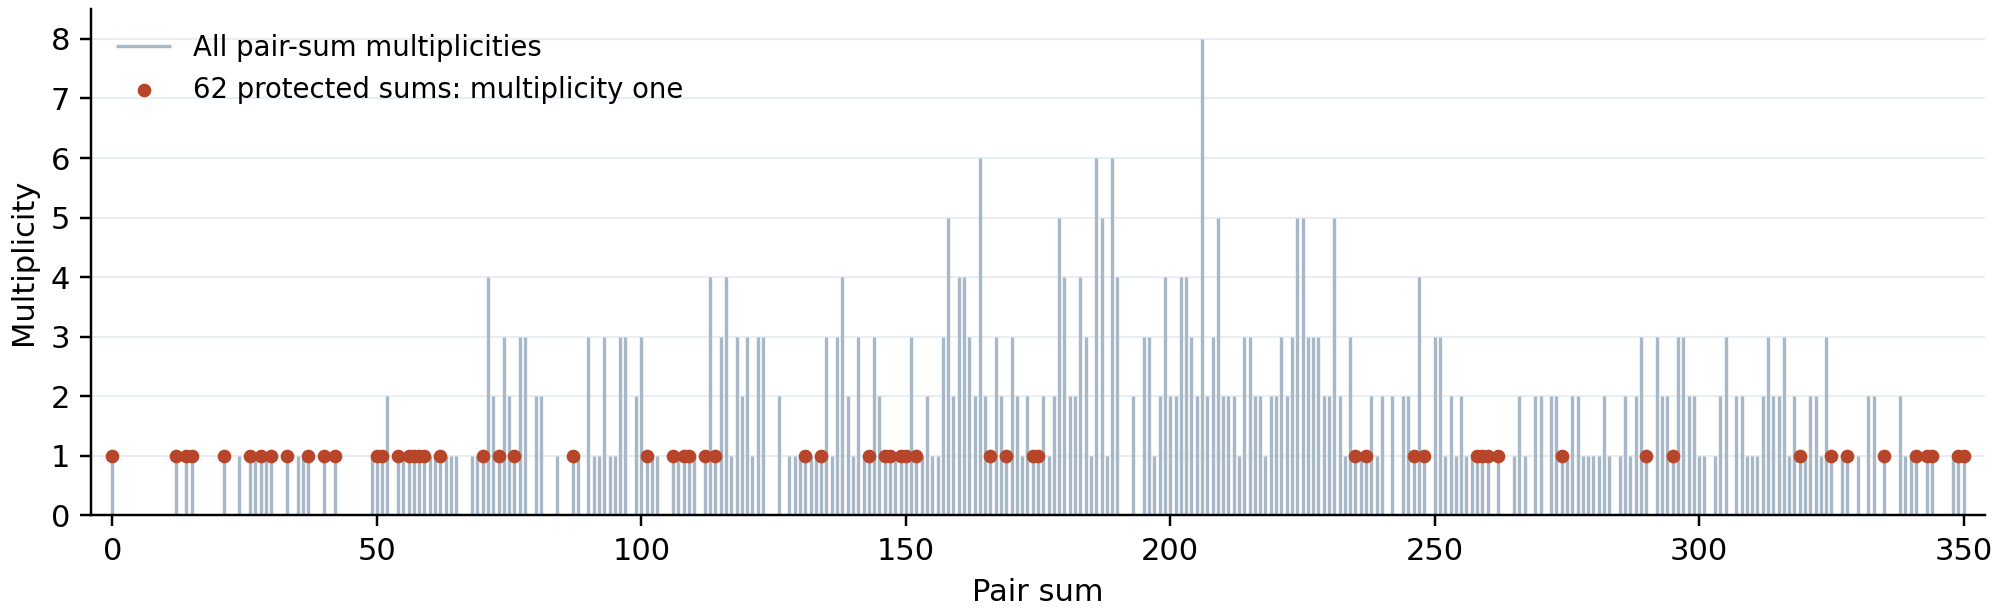
\includegraphics[width=\linewidth]{assets/pair_sums.png}
\caption{Pair-sum multiplicities of the explicit weights. Protected sums
have multiplicity one; unused sums may have larger multiplicity. The
certificate checks the full finite family, not just the displayed plot.}
\end{figure}

\subsection{Targets selected for actual supports}
For each original row, use the target and sign in Table~\ref{tab:targets}.
Only row 8 is negated. Write $\rho_j$ for the resulting signed residual
in increasing target order, and $E_j$ for its target.
\begin{table}[ht]
\centering
\begin{tabular}{rrr@{\qquad\qquad}rrr}
\toprule
Original row & Sign & Target & Original row & Sign & Target\\
\midrule
16 & $+$ & 246 & 13 & $+$ & 2721\\
17 & $+$ & 429 & 14 & $+$ & 3063\\
18 & $+$ & 657 & 12 & $+$ & 3312\\
21 & $+$ & 868 & 4 & $+$ & 3506\\
6 & $+$ & 1058 & 22 & $+$ & 3798\\
2 & $+$ & 1358 & 11 & $+$ & 3989\\
19 & $+$ & 1550 & 20 & $+$ & 4179\\
7 & $+$ & 1734 & 5 & $+$ & 4367\\
3 & $+$ & 2058 & 15 & $+$ & 4623\\
9 & $+$ & 2248 & 10 & $+$ & 4817\\
1 & $+$ & 2545 & 8 & $-$ & 5148\\
\bottomrule
\end{tabular}
\caption{Exact target assignment for the 22 original quadratic residuals.}
\label{tab:targets}
\end{table}


Write $e(\alpha)=\sum_i\alpha_iw_i$ and let
$\mathcal Q=\{w_a+w_b:0\le a\le b\le31\}$.
The certificate checks, for every supported monomial of row $i$ and
every distinct target row $j$,
\begin{equation}
E_j-E_i\notin\mathcal Q-e(\alpha).
\label{eq:cross}
\end{equation}
It also checks $E_i-e(\alpha)\ge0$. All 1,974 cross-row exclusions pass.
No uniform gap of $2t+1$ is required.

With $\rho_j(\mathbf p)=\sum_\alpha a_{j,\alpha}\mathbf p^\alpha$, define
\begin{equation}
\Dc(Z)=\sum_{j,\alpha}
\underbrace{(2-|\alpha|)!\prod_i\alpha_i!\,a_{j,\alpha}}_{c_{j,\alpha}}
Z^{E_j-e(\alpha)}.
\label{eq:kernel}
\end{equation}
The sum has exactly 94 distinct powers of $Z$. Its least exponent is 0,
its greatest is $E_*=5148$, and its leading coefficient is 2.
The last fact follows because the last row is
$P(P-k)+1-\tau^2$, whose constant is 1.

\begin{lemma}[Exact simultaneous extraction]
For independent indeterminates $p_1,\ldots,p_{31}$, put
\[
\mathcal C_{\mathbf p}(Z)=\left(1+\sum_{i=1}^{31}p_iZ^{w_i}\right)^2.
\]
Then for every $j$,
\begin{equation}
[Z^{E_j}]\,\mathcal C_{\mathbf p}(Z)\Dc(Z)=2\rho_j(\mathbf p).
\label{eq:extract}
\end{equation}
\end{lemma}
\begin{proof}
At a protected exponent $e(\alpha)$, selective isolation makes the
coefficient of $\mathcal C_{\mathbf p}$ exactly
$2!\mathbf p^\alpha/((2-|\alpha|)!\prod_i\alpha_i!)$.
This cancels the factorial multiplier in~\eqref{eq:kernel}.
Condition~\eqref{eq:cross} excludes every contribution from another row.
These two statements account for every term of the convolution.
\end{proof}

Different records in~\eqref{eq:kernel} cannot have the same exponent.
Within a row this follows from selective isolation. Across rows an overlap
$E_i-e(\alpha)=E_j-e(\beta)$ would give the forbidden difference
$E_j-E_i=e(\beta)-e(\alpha)$, with $e(\beta)\in\mathcal Q$.
Consequently coefficient bounds do not acquire a factor of 22.

\subsection{A shift of one word replaces 31 expanded substitutions}
If a nonnegative digit word is $g=\sum n_i\BB^{w_i}$, define
$\ell=\sum\BB^{w_i}$. Then
\begin{equation}
1+\ell+g=1+\sum_i(n_i+1)\BB^{w_i}.
\label{eq:wordshift}
\end{equation}
Thus one addition of $\ell$ evaluates the original parent at positive
coordinates $p_i=n_i+1$. Expanding $r_j(\mathbf n+\mathbf1)$ before
packing is unnecessary. That earlier expansion created 71 protected
monomials, 136 coefficient records, and 17 nontrivial recipes. Retaining
the raw parent leaves 62, 94, and 9 respectively.

\subsection{Removing common padding}
An initial valid target arrangement had first target 350 and last target
5252, with every kernel exponent at least 104. Subtracting 104 from all
targets preserves all differences in~\eqref{eq:cross}. It gives the
displayed targets 246 through 5148 and makes the least kernel exponent
zero. This is the maximal common translation for that arrangement.

The old package-40 product span was $36\,775$. The new one is
\begin{equation}
M=E_*+2t=5498.
\label{eq:span}
\end{equation}
The search is a discovery tool; only the finite list and its checked
properties are premises of the proof. No optimality of span 175 or of
the target arrangement is required.

\section{A complete source for the ten-integer construction}
\label{sec:source}

Use the conservative fixed bound
\[
H_0=8(1+\beta+K_0+M_C+M_F)^2,
\qquad \beta_S=2^{2\,140\,030}.
\]
The finite audit finds ordinary coefficient $\ell^1$-norm at most 4 and
port degree at most two. Hence $|a_{j,\alpha}|\le H_0$ and each kernel
coefficient has absolute value at most $2H_0$. Exact integer arithmetic
verifies
\begin{equation}
\beta_S>4\cdot33^2H_0.\label{eq:betabound}
\end{equation}
The bit lengths of $H_0$ and $4\cdot33^2H_0$ are $2\,140\,010$ and
$2\,140\,022$, respectively. The even exponent of $\beta_S$ also ensures
$\beta_S\equiv1\pmod3$.

The letters below refer to the ten final unknowns, independently of
similarly named parent coordinates. With integer $f,g$, define
\begin{align}
b&=1+3f,&\BB&=\beta_Sb^2,&\ell&=\sum_i\BB^{w_i},\notag\\
N_0&=\BB^{176},&N_1&=4\BB^{5499},&N&=N_0N_1,\notag\\
M_c&=N_0-1-(b-1)\ell,&Q_c&=(\BB-2)\sum_j\BB^{E_j},\notag\\
T_c&=M_c+Q_cN_0,&&&\notag\\
J_c&=2(1+\ell+g)^2\Dc(\BB)+\BB\sum_{r=0}^{5498}\BB^r,&&&\notag\\
S_c&=g+J_cN_0,&R_c&=(S_c+T_c+1)N+T_c+1,\notag\\
X&=(N-1)R_c,&Y&=N^2,&\Ccap&=b\BB^{175}.
\label{eq:source}
\end{align}
All sums and powers have fixed limits. In particular,
\[
N=4\BB^{5675},\qquad
\Ccap=2^{374\,505\,250}b^{351}.
\]
The latter has exactly the even power-of-two coefficient and odd
$b$-exponent required by the inherited ten-integer bridge.

\begin{proposition}[Source interface]
\label{prop:source}
The following statements hold.
\begin{enumerate}[label=(\roman*)]
\item If the positive parent has a solution, then for every sufficiently
large positive $f$ with $b$ a square and a power of two there is an integer
$g$ such that $b\le g<\Ccap$ and $Y\mid\binom{2X}{X}$.
\item If $f\ne0$, $b$ is a square and a power of two,
$0\le g<2\Ccap$, and $Y\mid\binom{2X}{X}$, the positive parent has a solution.
\item Already if $f\ne0$, $b$ is a square, and $0\le g<2\Ccap$, without
assuming it is a power of two, one has
$0\le S_c,T_c<N$, $3\mid X$, $X>3b$, and $Y>\max(b,256)$.
\end{enumerate}
\end{proposition}

\subsection{Bounds before digit recovery}
If $b=1+3f$ is a square and $f\ne0$, then $f>0$, $b\ge4$, and
$\BB>2b$. Since the kernel has leading coefficient 2 and all other
coefficients bounded by $2H_0$,
\[
\Dc(\BB)\ge2\BB^{E_*}-2H_0\sum_{r<E_*}\BB^r>0.
\]
Its absolute value is at most $2H_0\sum_{r=0}^{E_*}\BB^r$.
Distinct positive weights give $1+\ell<2\BB^t$; hence for the full
permitted interval $0\le g<2b\BB^t$,
\[
1+\ell+g<3b\BB^t.
\]
It follows from~\eqref{eq:betabound} that
\begin{align*}
0<J_c
&\le(36H_0b^2+\BB)\sum_{r=0}^M\BB^r\\
&<2\BB^{M+1}<N_1,
\end{align*}
where $36H_0b^2\le\BB-2$ suffices. Also $g<N_0$, so $0<S_c<N$.
The mask digits give $0\le M_c<N_0$; likewise
$0\le Q_c<\BB^{E_*+1}<N_1$, yielding $0\le T_c<N$.

Since $b\equiv\beta_S\equiv1\pmod3$, one has $N\equiv1\pmod3$,
and thus $3\mid X$. Moreover $R_c\ge N+1>\BB>b$ and $N\ge4$ imply
$X>3b$. The chosen base gives $Y>\max(b,256)$. This proves (iii).
The ordering of this argument matters: the arithmetic bridge recovers
that $b$ is a power of two only after these range estimates are available.

\subsection{Two exact carry tests}
Now assume $b$ is a power of two. Then $\BB,N_0,N$ are powers of two.
For nonnegative integers let
\[
\tau_2(u,v)=\pc(u)+\pc(v)-\pc(u+v)
\]
be the number of binary carries, counted with multiplicity. Its vanishing
means that the binary supports of $u$ and $v$ are disjoint.

The low mask $M_c$ has digit $\BB-b$ at the 31 weights and $\BB-1$
elsewhere below $N_0$. Therefore
\begin{equation}
\tau_2(g,M_c)=0\quad\Longleftrightarrow\quad
g=\sum_i n_i\BB^{w_i},\quad 0\le n_i<b.
\label{eq:lowmask}
\end{equation}
Set $p_i=n_i+1$. The coefficients of $\mathcal C_{\mathbf p}\Dc$ have
absolute value at most $2H_0(1+\sum p_i)^2<\BB/2$ by
$p_i\le b$ and~\eqref{eq:betabound}. Consequently
\[
K_c=(1+\ell+g)^2\Dc(\BB)+\frac{\BB}{2}\sum_{r=0}^{M}\BB^r
\]
has ordinary base-$\BB$ digits strictly between 0 and $\BB$. The digit
at target $E_j$ is $\BB/2+2\rho_j(\mathbf p)$.
For such a digit $d$, disjointness from $\BB/2-1$ is equivalent to
$d=\BB/2$. Since $J_c=2K_c$ and
$Q_c=2(\BB/2-1)\sum_j\BB^{E_j}$, a common binary shift gives
\begin{equation}
\tau_2(J_c,Q_c)=0\quad\Longleftrightarrow\quad
\rho_1(\mathbf p)=\cdots=\rho_{22}(\mathbf p)=0.
\label{eq:highmask}
\end{equation}
Division by two appears only in this proof, not in the final circuit.
Low and high blocks are disjoint, so the conjunction of
\eqref{eq:lowmask} and~\eqref{eq:highmask} is exactly
$\tau_2(S_c,T_c)=0$.

\begin{lemma}[Central-binomial carry identity]
If $N=2^e$ and $0\le S,T<N$, then
\[
N^2\mid\binom{2X}{X}\quad\Longleftrightarrow\quad\tau_2(S,T)=0,
\qquad X=(N-1)((S+T+1)N+T+1).
\]
\end{lemma}
\begin{proof}
The exact block expansion is
\[
X=(S+T)N^2+(N-1-S)N+(N-1-T).
\]
The lower blocks are $e$-bit complements. Thus
$\pc(X)=2e-\tau_2(S,T)$, while Legendre's factorial formula gives
$\nu_2\binom{2X}{X}=\pc(X)$. Since $\tau_2\ge0$, divisibility by
$2^{2e}$ is equivalent to its vanishing.
\end{proof}

This proves the reverse source implication. For the forward implication,
start with a positive parent solution $\mathbf p$, choose an arbitrarily
large $b=2^{2q}>\max p_i$, and set $f=(b-1)/3$ and
$g=\sum(p_i-1)\BB^{w_i}$. The all-one parent assignment is not a zero:
its fifth residual is 1. Thus $g\ge\BB>b$. Also
\[
g\le(b-1)\sum_{j=1}^{t}\BB^j<b\BB^t=\Ccap,
\]
because $b<\BB$. Both carry tests pass. This proves
Proposition~\ref{prop:source} in full.

\section{The single equation in ten unrestricted integers}
\label{sec:ten}

Use exactly the ten integer unknowns
\[
f,g,h,k,l,w,x,y,z,m.
\]
Starting with~\eqref{eq:source}, define the following polynomial
abbreviations. They are the inherited Sun/package-31 finalizer
\cite{sun2026,package31,package40} with the newly proved source substituted:
\begin{align}
L&=lY,&U&=2LX,&V&=4gwY,&W&=bw,\notag\\
A&=U(V+1),&B_1&=2X+1,&C&=B_1+(A-2)h,\notag\\
P_n&=U^2V,&K&=X+1+k(P_n-2),\notag\\
S&=2A-5,&T&=3WC-2(W^2-1),\notag\\
R_2&=(P_n^2-4)K^2+4.&&&&\label{eq:tenbridge}
\end{align}
Next put
\begin{align}
\Delta_b&=8\Ccap^3gK^2-g^2\bigl(32(C-KL)^2\Ccap^3+g^2K^2\bigr),\notag\\
O&=f^2l^2\Delta_b,\qquad \xi=zx,\notag\\
D&=(A^2-4)C^2+4,\qquad E=C^2D\xi,\notag\\
F&=4(A^2-4)E^2+1,\notag\\
G^*&=2(A+2)(A-2)^2E^2-1,\qquad\Omega_0=16E,\notag\\
H^*&=C+(B_1-C)F+\Omega_0Fy,\notag\\
I^*&=((G^*)^2-1)(H^*)^2+1.\label{eq:tenlucas}
\end{align}
The divisibility merger and radicands are
\begin{align}
\Sigma&=\xi S^5,&r&=T+Sy,\notag\\
\Theta&=(r^3-rS^2-S^3)(r^2+23S^2),\notag\\
r_0&=b\bigl(1+(3O-4)b^2z^2\bigr),&r_1&=R_2,&r_2&=DFI^*,\notag\\
v_1&=r_0,&v_2&=r_0(P_n^2+K^2+3).
\label{eq:tenrad}
\end{align}
Finally define
\begin{align}
Z&=\Sigma m-\Theta,\notag\\
a_0&=\Sigma^2r_0,&a_1&=\Sigma^2v_1^2r_1,&a_2&=\Sigma^2v_2^2r_2,\notag\\
V_n&=Z^2+a_2-a_0-a_1,&W_n&=V_n^2+4Z^2a_2-4a_0a_1.
\label{eq:tennorm}
\end{align}
The promised equation over \emph{all integers} is
\begin{equation}
\boxed{\quad P_{10}=W_n^2-16V_n^2Z^2a_2=0.\quad}
\label{eq:tenfinal}
\end{equation}
There are no roots, variable exponents, order predicates, or hidden
parameters in this polynomial. The coefficient kernel~\eqref{eq:kernel},
the explicit weights and targets, and the four fixed payloads determine
every coefficient. The literal circuit is \file{data/polynomial.json}.

\section{Proof that the finalizer preserves solvability}
\label{sec:tenproof}

The numerical Lucas and binomial bridges are inherited from Sun's 2021
paper and 2026 preprint \cite{sun2021,sun2026}. Their use here is through
their proofs with the source interface replaced by
Proposition~\ref{prop:source}, as in package 40. All required source properties
are now established: arbitrarily large square dyadic bases, the two
binomial implications, the broad range bounds, $b=1+3f$, the stated
congruences and sizes, and $\Ccap=2^c b^d$ with fixed even $c$ and odd $d$.
No old quartic digit identity is used after that substitution.

\subsection{The exact bridge obligations}
Let $u_n(A)$ be the Lucas sequence $u_0=0,u_1=1$,
$u_{n+1}=Au_n-u_{n-1}$, extended to integer indices. The cited bridge
gives these implications for~\eqref{eq:tenbridge}--\eqref{eq:tenlucas}:
\begin{enumerate}
\item A positive parent solution yields witnesses with $A>2$ even,
$B_1>0$ odd, $b$ square, $b\le g<\Ccap$, $C=u_{B_1}(A)$,
$R_2$ square, $S\mid T$, and $O>0$.
\item Conversely, $b$ square, $O>0$, $\xi\ne0$, $DFI^*$ square,
$R_2$ square, and $S\mid T$ imply a positive parent solution.
\item If $A>2$ is even, $B_1>0$ is odd, and $C=u_{B_1}(A)$,
then for every positive modulus divisor $d$ one can choose $\xi>0$
divisible by $d$ so that every residue class modulo $\xi$ contains a
$y$ for which $DFI^*$ is a square.
\end{enumerate}
The last statement is Sun's full residue-class interpolation theorem.
In the reverse direction, $O>0$ first gives $f,l\ne0$, $g>0$,
$K\ne0$, $g<2\Ccap$, and $4(C-KL)^2<K^2$. The broad source bounds
then make the Lucas reverse theorem applicable. It recovers
$W=2^{B_1}$ and the binomial divisibility; since $W=bw$ with $b>0$,
it also recovers that $b$ is a power of two. This avoids assuming the
digit interpretation before it has been justified.

\subsection{Divisibility and nonvanishing in one expression}
The quintic
\[
\pi(v)=(v^3-v-1)(v^2+23)
\]
has a root modulo every positive integer but no rational root. For an odd
prime other than 23, either the cubic has a simple root, or it is
irreducible and its discriminant $-23$ is a square, so the quadratic
has a simple root. At 23 the cubic has the simple root 3. At 2,
$-23\equiv1\pmod8$ is a square in $\Z_2$. Hensel lifting and the
Chinese remainder theorem give roots modulo arbitrary positive integers.
The rational-root test and positivity of $v^2+23$ exclude rational zeros.

The odd integer $S=2A-5$ is nonzero. If $S\mid T$, writing $T=Sq$ gives
$\Theta=S^5\pi(q+y)$. A root of $\pi$ modulo $|\xi|$ therefore permits
a residue class of $y$ with $\Sigma\mid\Theta$.
Conversely, if $S^5\mid\Theta$ but $S\nmid T$, choose a prime with
$\nu_p(S)=\alpha>\beta=\nu_p(T)$. The two homogeneous factors of
$\Theta$ have valuations $3\beta$ and $2\beta$, contradicting
$5\alpha\le\nu_p(\Theta)$. Also $\Theta\ne0$, since otherwise
$(T+Sy)/S$ would be a rational root of $\pi$.

\subsection{The square and positivity conditions}
For $z\ne0$, if $r_0$ is a square then $b$ and
$1+(3O-4)b^2z^2$ are coprime. The second factor cannot be zero: that
would force $|b|=|z|=1$, hence $b=1$, $f=O=0$, a contradiction.
Unique factorization makes $b$ a signed square. A negative nonzero square
is not 1 modulo 3, so $b$ is a positive square. If $O\le0$, the other
factor is at most $1-4(bz)^2<0$, impossible. Thus $O>0$.

Conversely, positive bridge witnesses have $O\ge g\ge b\ge4$.
The positive nonsquare $3O-4\equiv2\pmod3$ has a Pell unit. Raising a
positive unit to a suitable finite order modulo $b$ produces
$u^2-(3O-4)v^2=1$ with $v>0$ divisible by $b$. Taking $z=v/b$ makes
$r_0$ a square. Interpolation subsequently chooses $\xi$ divisible by
$z$, so $x=\xi/z$ is an integer. Its residue-class clause allows the
same $y$ to satisfy the quintic merger and the Lucas square condition.

\subsection{A separating norm detects all three squares}
For every assignment with $z\ne0$, one has $|r_0|>1$. Indeed
$r_0\in\{0,1,-1\}$ would force $|b|=1$, hence $b=1,f=O=0$,
but then $r_0=1-4z^2\le-3$. Also
\[
\sqrt{|r_1|}\le P_n^2+K^2+2.
\]
Squaring this bound and subtracting $(P_n^2+4)K^2+4$ leaves
$P_n^4+K^4+P_n^2K^2+4P_n^2\ge0$. Consequently
\begin{align*}
|v_1|&>\sqrt{|r_0|},\\
|v_2|&>\sqrt{|r_0|}+|v_1|\sqrt{|r_1|}.
\end{align*}
If a signed weighted sum of the roots of $r_0,r_1,r_2$ is rational,
all three roots must be rational. Otherwise take a Galois automorphism
changing a root and consider the largest-index changed nonzero term.
Its change dominates the sum of all earlier changes by these inequalities.
The argument uses complex absolute values and also covers negative radicands.
Rational square roots of integers are integer roots, so every radicand is
a nonnegative square.

The exact identity
\begin{equation}
W_n^2-16V_n^2Z^2a_2=
\prod_{\varepsilon\in\{-1,1\}^3}
\left(Z+\varepsilon_0\sqrt{a_0}
        +\varepsilon_1\sqrt{a_1}+\varepsilon_2\sqrt{a_2}\right)
\label{eq:normidentity}
\end{equation}
follows by repeated multiplication of conjugates; the radicals cancel.
An independent sparse expansion checks all 35 terms of the resulting
degree-eight polynomial.

Given a positive parent solution, the preceding construction makes all
$r_i$ squares and ensures $\Sigma\ne0$, $\Sigma\mid\Theta$. Choose $m$
so that one factor of~\eqref{eq:normidentity} vanishes. Conversely,
if~\eqref{eq:tenfinal} holds and $\Sigma=0$, its left side is
$\Theta^8\ne0$, a contradiction. Thus $\xi=zx\ne0$. A vanishing norm
factor divided by $\Sigma$ is a rational weighted root sum. Separation
makes all $r_i$ squares, and integrality gives $\Sigma\mid\Theta$.
The merger gives $S\mid T$, and the coprime argument gives $b$ square and
$O>0$. The reverse bridge and Proposition~\ref{prop:source} now recover
the parent solution. Composition with the inherited parent theorem proves
\eqref{eq:main10}.

\section{Exact degree, circuit size, and what the audits prove}
\label{sec:audit}

The main circuit has 422 multiplication gates, 138 addition gates, and
80 subtraction gates. Every counted gate is reachable from its output;
all ten input variables occur. Fixed powers are expanded into binary
multiplications. Reuse is free, coefficient leaves are fixed inputs, and
every binary operation in the delivered evaluator is counted.

The main source degrees are
\[
\deg X=34050,\qquad \deg Y=22700,\qquad\deg\Ccap=351.
\]
The inherited finalizer degree computation gives
\begin{equation}
456(34050)+896(22700)+24(351)+1760=35\,876\,184.
\label{eq:degree10}
\end{equation}
This is independently certified on the actual DAG: degree propagation
provides an upper bound, and after all ten variables are replaced by one
indeterminate $T$, the coefficient at that bound is
\[
[T^{35\,876\,184}]P_{10}(T,\ldots,T)
\equiv996362474\pmod{1\,000\,000\,007}.
\]
The nonzero residue proves a matching lower bound. This is exact
coefficient arithmetic, not a random evaluation used to infer degree.

\begin{center}
\begin{tabular}{p{0.32\linewidth}p{0.60\linewidth}}
\toprule
Claim & Evidence\\
\midrule
Raw parent records & Symbolic reconstruction from all 22 original residuals,
with the four ports left indeterminate.\\
Selective extraction & Exact symbolic equality of all 22 target
coefficients, including all cross-row exclusions.\\
Fixed coefficients & Payload hashes, bit lengths, coherent tuple binding,
exact coefficient bound, and complete reconstruction from the literal K215 transitions.\\
Final norm identity & Independent 35-term sparse polynomial expansion.\\
Operation count and exact degree & Full DAG liveness and degree/leading
coefficient certificates.\\
Literal source/finalizer implementation & Independent modular replay of
the stated formulas at signed sample inputs; diagnostic support in addition
to the mathematical derivation.\\
Unbounded solvability equivalence & The new source proofs, the stated
arithmetic bridges, and the inherited positive-parent theorem.\\
\bottomrule
\end{tabular}
\end{center}

The auditors also reject deliberately changed weights and targets. The
finite audits pass both normally and with Python optimization enabled.
They do not search for a solution, prove consistency, or replace an
unbounded compiler theorem. The distinction between exact symbolic checks
and diagnostic sample replay is explicit in the receipts.

\section{Nine positive unknowns: a second improved equation}
\label{sec:nine}
The same support-selective source also improves the nine-variable Jones
route.  Its primary circuit has nine strictly positive unknowns, exact
total degree $19\,615\,180$, and $606$ binary arithmetic operations.  The
equivalent version over nonnegative integers uses $609$ operations.  The
previous package-45 positive equation has degree $129\,875\,980$ and $788$
operations.  This is a reduction of approximately $84.9\%$ in degree and
$23.1\%$ in operations, without changing the number of unknowns.

Let the raw quadratic source, its weights and its targets be as above, and
write $W=175$, $H=5148$, and $K=H+2W=5498$.  Set
$M=2^{2140017}$ and $b_0=2^{2140030}=8192M$.  Initially take
$\epsilon,\phi,n\geq0$ and $g,h,s,w,i,j>0$. Define
\begin{align*}
b&=b_0+\epsilon,& B&=b^3,& \ell&=\sum_{r=1}^{31}B^{w_r},\\
N_0&=B^{W+1},&N_1&=4B^{K+1},&N&=N_0N_1,\\
L&=N_0-1-(b-1)\ell,& Z&=\sum_{r=1}^{22}B^{E_r},\\
T&=L+(B-2)ZN_0,&&&\\
J_0&=2(1+\ell+g)^2\Dc(B)+B\sum_{r=0}^{K}B^r,&&&\\
S&=g+J_0N_0,&R&=(N-1)((S+T+1)N+T+1),\\
G_{\mathrm{cap}}&=32bB^W.&&&
\end{align*}
Every exponent is fixed.  The raw residuals are evaluated at positive
digits $x_r=z_r+1$: the one added $\ell$ implements all thirty-one
positivity shifts in the common convolution factor.

The coefficient at the largest exponent of $\Dc$ is $2$, and all its other
coefficients have absolute value below $M$. Hence $\Dc(B)>0$ unconditionally.
The source therefore satisfies $R,N\geq8$ and $b\leq R,N$ before any
equation is imposed. If $g<4bB^W$, then $1+\ell+g<5bB^W$, and the choice
$b\geq8192M$ gives $0<S,T<N$.  With $b$ a power of two, the exact
population-count identity
\[
\operatorname{popcount}(R)=2\log_2N+
\operatorname{popcount}(S+T)-\operatorname{popcount}(S)
-\operatorname{popcount}(T)
\]
shows that $N^2\mid\binom{2R}{R}$ is precisely the no-carry condition.
Its low block encodes $g=\sum z_rB^{w_r}$ with $0\leq z_r<b$; its target
blocks impose all the original positive quadratic equations simultaneously.
Conversely, every positive parent solution permits arbitrarily large
dyadic bases with $32g<G_{\mathrm{cap}}$.  The all-one parent assignment
is not a zero, because its residual $a-E-sN$ equals $-1$, so $g>0$.

All the numerical Jones bridge registers are as follows
\cite{package45,jones}. The names $K_1,D_1,H_1$ distinguish these
registers from the source exponent bound $K$, kernel $\Dc$, and maximum
target $H$:
\begin{align*}
U&=N^2w,&Y_0&=N^2s,&M_0&=RY_0,\\
P&=2M_0^2U,&K_1&=R+1+h(P-1),&A&=M_0(U+1),\\
B_1&=2R+1,&W_1&=bw,&C&=B_1+W_1+\phi,\\
J&=4A-5,&Q&=3W_1C-2(W_1^2-1),&&\\
D_1&=(A^2-1)C^2+1,&E&=iJD_1C^2,&&\\
F&=(A^2-1)E^2+1,&G&=A+F(CD_1+1-A),&&\\
H_1&=B_1+jC,&I&=(G^2-1)H_1^2+1,&&\\
a_0&=(P^2-1)K_1^2+1,&a_1&=D_1FI,&&\\
u&=JF,&v&=QF+J(H_1-C).&&
\end{align*}
Define the margin polynomial
\[
m=K_1^2G_{\mathrm{cap}}
 -4(C-K_1Y_0)^2G_{\mathrm{cap}}-8gK_1^2.
\]
Here $m$ is a polynomial register, not a tenth unknown.

The hypotheses of \texttt{Jones1982.Nine.ratio\_sound} and
\texttt{ratio\_complete} are $R,N\geq8$, $b\leq R,N$,
$b,G_{\mathrm{cap}}>0$, $h,s,w,i,j>0$ and $\phi\geq0$.
All have been supplied independently of the carry condition.
Soundness states that $a_0,a_1$ squares, $u\mid v$, and $m>0$ imply
that $b$ is a power of two, $N^2\mid\binom{2R}{R}$, and
$8g<G_{\mathrm{cap}}$. The latter is exactly $g<4bB^W$, the
interval needed by the source. Completeness starts with $b$ a power
of two, the divisibility, and $32g<G_{\mathrm{cap}}$, and supplies
$h,s,w,i,j,\phi$ satisfying the four arithmetic conditions.
This is precisely the stronger interval supplied by a parent zero.
No property of the Sun ten-integer bridge is used here.

Set
\[
V_0=PK_1,\qquad V_1=(AC)(AE)(GH_1),\qquad M_d=Q+H_1.
\]
These registers are positive. The identities
\begin{align*}
V_0^2-a_0&=K_1^2-1>0,&(AC)^2-D_1&=C^2-1>0,\\
(AE)^2-F&=E^2-1>0,&(GH_1)^2-I&=H_1^2-1>0
\end{align*}
give $0<a_0<V_0^2$ and $0<a_1<V_1^2$ on every outer assignment.
Also $Q>0$, $H_1-C>0$, and
$0<v/u=Q/J+(H_1-C)/F<M_d-1$.

One polynomial combines these four conditions. Put
\[
\Omega=um,\qquad
\Theta=u(n+M_d)+v-\Omega(2M_d+V_0V_1),
\]
and take
\[
\boxed{\bigl(\Theta^2-\Omega^2(a_0+V_0^2a_1)\bigr)^2
       -4\Omega^4V_0^2a_0a_1=0.}
\]
At $m=0$ its left side is nonzero. Otherwise its four-factor norm identity
implies that a rational number is $r_0+V_0r_1$, with $r_t^2=a_t$.
The strict majorant excludes a zero rational sum; the identity
$2(r_0+V_0r_1)r_0=(r_0+V_0r_1)^2+a_0-V_0^2a_1$ then makes both roots
integers. Their bounds give
$2M_d+V_0V_1+r_0+V_0r_1\geq2M_d+1>0$, which forces $m>0$ and
$u\mid v$.  The converse chooses $n$ from this same positive expression.
Thus this finalizer has both the required soundness and completeness.

To define the polynomial on nine \emph{positive} coordinates, replace
$\epsilon,\phi,n$ throughout by their positive coordinates minus one,
leaving $g,h,s,w,i,j$ positive. For the nine \emph{nonnegative} version,
instead leave $\epsilon,\phi,n$ unchanged and replace each of
$g,h,s,w,i,j$ by its nonnegative coordinate plus one. These are bijections
with the mixed domain used in the proof. They establish the stated
solvability equivalences; they do not justify an unrestricted-integer
interpretation of this nine-variable equation.

The full exact degree is
\[
1152t+12W+280=19\,615\,180,
\qquad t=3(H+3W+2)=17\,025.
\]
The cancellation-resolved circuit proves this upper bound, and its
all-variable diagonal has nonzero leading coefficient $2^{2050}$, proving
equality. Its critical exact identity is
\begin{align*}
\Delta_V=V_1^2-a_1
 ={}&(C^2-1)(AE)^2(GH_1)^2\\
   &+D_1(E^2-1)(GH_1)^2+D_1F(H_1^2-1).
\end{align*}
Writing $E_0=u(n+M_d)+v-2\Omega M_d$, the inner polynomial of the
final equation equals
\[
E_0^2-2E_0\Omega V_0V_1+\Omega^2V_0^2\Delta_V-\Omega^2a_0.
\]
Its uniquely highest degree is $576t+6W+140$, with diagonal coefficient
$2^{1025}$. The final subtracted term has smaller degree than its square.
The full proof is in \file{nine/PROOF.md}; the polynomial identity is
independently replayed by the verifier. The source is explicit, while the
finite audits are implementation checks, not a decision of consistency
or a new end-to-end formal proof of the inherited compiler.


\section{Reproducibility, formalization, and remaining opportunities}
\label{sec:reproduce}

The archive is self-contained for all newly introduced finite algebra and
circuit checks. It includes this LaTeX source and compiled PDF, literal
circuits for both domains, fixed coefficient bytes and recipes, the raw
parent, inherited proof excerpts and notices, source hashes, and independent
audit programs. The main commands from the extracted package root are
\begin{verbatim}
python3 verify.py
python3 code/build.py
python3 code/audit_candidate.py
python3 nine/build_nine.py
python3 nine/verify_nine.py
pdflatex -interaction=nonstopmode -halt-on-error report.tex
pdflatex -interaction=nonstopmode -halt-on-error report.tex
\end{verbatim}
The first command performs the finite release checks in a temporary copy.
The manuscript can be incorporated as a new report directory while
preserving the supplied licenses and pinned provenance.

The most useful next formalization step is the generic selective extraction
lemma with a finite certificate as input. Its proof is a short multinomial
coefficient calculation plus finite noninterference conditions. A second
small module can prove the single-word positivity substitution. Those
lemmas can be linked to the existing data-valued compiler infrastructure
without using a proposition-valued existence theorem to fabricate
executable coefficient data.

The main unresolved end-to-end proof-assistant task remains the inherited
native-window compiler bridge. A checked arithmetic equivalence about
syntactic ZFC consistency is also distinct from a derivation in the
object-language ZFC proof calculus. This report supplies ordinary
mathematical reductions intended for that formalization; it does not
relabel either open task as completed.

There remain concrete optimization problems: jointly choosing selective
weights and targets, exploiting equality of coefficient vectors rather
than requiring every supported exponent to be unique, and choosing a
different sparse quadratic parent. The certificate formulation makes such
experiments inexpensive to validate. Any future reduction must continue
to check all unused monomial contamination and all broad witness bounds.
Those two requirements are essential to the present proof.

\appendix
\section{A modest additional local degree-68 improvement}
\label{app:p74}

The active repository's checked 75-operation degree-68 polynomial uses
fifteen positive variables and the six factors $N_0,N_1,N_a,N_k,N_t,N_s$
of its \file{SHORT_SYSTEM.md}. Its equation is
\[
(N_0-1)^2+(N_a-1)^2+(N_s-1)^2+(N_1N_kN_t-1)^2=0.
\]
A new local alternative is
\begin{equation}
N_0^2+N_a^2+N_s^2+(N_1N_kN_t-1)^2-3=0.
\label{eq:p74}
\end{equation}
It has the same positive zero set and costs 74 operations at the same
exact degree 68. This is a one-gate local improvement, separate from the
main low-variable construction.

The reason is that $N_0,N_a,N_s$ are nonzero before any equation is
assumed. The first and third are norms with nonsquare discriminants
$n(n+1)$ and $(a+2)^2-1$, and their relevant positive coordinates are
nonzero. For the middle factor write
$N_a=A V^2-(A-1)y^2$ with $A=\Delta(f^2-1)$. If $f=1$, it equals
$y^2>0$. Otherwise $A\ge2$; a zero would make the reduced fraction
$(A-1)/A$ a rational square, forcing both consecutive positive integers
$A-1,A$ to be squares, impossible.

Thus the first three squares in~\eqref{eq:p74} are at least one; equality
forces each to be one and forces $N_1N_kN_t=1$. The inherited negative
Pell and modulo-four unit-sign arguments force $N_0=N_a=N_s=1$.
Conversely those values make~\eqref{eq:p74} vanish. Only $N_s^2$ reaches
degree 68, with leading form
\[
i^4w^4s^{12}(\eta+\zeta)^8(\beta J)^{40}.
\]
The local JSON, proof, and finite audit are supplied under \file{short/}.
This is an ordinary local proof; it is not represented as a newly compiled
Lean theorem. Its source tuple and coordinate conventions are preserved
separately from the main package-31 construction.

\section{A smaller complete native coefficient tuple}
\label{app:coefficient-adapter}

A separate adapter in \texttt{coefficient\_adapter/} reduces the fixed
coefficient heights of the inherited K215 native/Pell interface:
\[
 \rho=2^{89},\qquad L=4831,\qquad B=\rho^L=2^{429959}.
\]
Its four raw coefficient ports occupy \(215\,492\) bytes, versus
source44's \(295\,388\) bytes for \(B=2^{590069}\), a reduction of
\(27.0478\%\). The base exponent decreases by \(27.1341\%\).
The port bit lengths, in order
\((\beta,K,M_C,M_{F,\mathrm{source}})\), are
\(429959,434054,429959,429960\).
The main low-variable equations in this article retain their source31
tuple. Substituting the new tuple would require rebuilding their
derived index constants.

\paragraph{The new mechanism.}
Source40 factors \(488\) receiver tiles into two modes and seventeen
Boolean payload bits, leaving \(457\) selector modes, but explicitly
leaves an empty-cell soundness obligation open. Source44 supplies
aggregate complement clauses. The new adapter combines these ideas
with complemented edge labels, doubled horizontal labels, and reuse
of the copied west parity bit as the current anchor. It removes four
dedicated occupancy copies and the separate current anchor; the support
has \(520\) native positions.

Put \(T=2^{42}\), \(M=4T\). The selector and gate masks give
\(n\in\{0,1\}\). For mode \(i=(w_i,n_i,e_i,s_i)\) and receiver payloads
\(Q_R,Q_L\in\{0,\ldots,255\}\), \(u\in\{0,1\}\), define
\[
 \begin{aligned}
 L_i&=2w_i+2^{11}n_i+2^{21}(2e_i)+2^{32}s_i,\\
 V&=2Q_R+2^{11}u+2^{21}(2Q_L)+2^{32}(2Q_R+2Q_L+u).
 \end{aligned}
\]
The label widths are \(11,10,11,10\). Let \(Z<T\) be the copied label
vector, \(y=Z\bmod2\) its west low bit, and \(A_1,A_2\) the two
standalone anchors. The same physical bit \(y\) is used twice:
\begin{equation}
 W=Z+T(y+A_1+A_2),\qquad
 \sum_i x_i(1+L_i)+V+W\equiv0\pmod M.                 \label{eq:adapterpayload}
\end{equation}
All coefficients are nonnegative. Every \(L_i,V\) is even, so \eqref{eq:adapterpayload}
gives \(y=n\).

If \(n=0\), then \(W<3T\) and \(V<T\). Hence \(0\le V+W<M\),
so \(V=W=0\): all payloads, copies and anchors vanish, apart from the
ignored dummy digits. This closes the old empty-cell gap.
If \(n=1\), the gates give \(0\le L_i+V<T\), and the positive sum in
\eqref{eq:adapterpayload} is less than \(2M\). It therefore equals \(M\), giving
\[
 W=3T+\bigl(T-1-(L_i+V)\bigr).
\]
Thus \(y=A_1=A_2=1\), and the copied labels are exactly complemented.
Both horizontal labels were doubled, so their complemented low bits
are one. Conversely every intended occupied encoding satisfies the
clause. This uniform interval argument supplies the local theorem.

\paragraph{The full native interface.}
The shared source anchor is the west copy at position \(539\);
the two tested temporal anchors remain \(1203,1807\). The bare shifts
are \(33,68,664,1268\), clause targets \(2409,3015\), and spatial
exponent \(46\). Complete basis identities and the two exact support
intersections give a clean Start clause, binary synchronization
including the upper-dummy exception, and whole-cell alignment.
Spatial matching then propagates occupation through the cyclic word:
an occupied east low bit is one, while the west low bit equals \(n\).
Complementation and doubling preserve edge matching. Deleting the
\(536\) unmatched receiver expansions recovers the original marked
K215 Wang language.

The masks have populations \(520\) and \(429959-520\), with the same
required low congruences as the source interface. All conservative
carry and strict-slack thresholds are below \(2^{89}\).
Completeness uses the fixed prime \(\lambda=106261\):
\[
 \operatorname{ord}_{429959}(B)=26565\mid(\lambda-1),
 \qquad B^{\lambda-1}\bmod\lambda^2=8376873414\ne1.
\]
The certified controller units allow the inherited Boolean dummy
adjustment of the actual packed rank. The full coefficient recipe,
synchronization proof, completeness argument and canonical witness
promises are in \texttt{SEPARATED\_PROOF.md}.

\paragraph{Verification and scope.}
The independent auditor imports neither builder and reconstructs the
Wang language from all \(430\) literal K215 actions. It verifies \(37\,960\) native basis
identities, \(1\,479\) occupied encodings, \(65\,076\) physical bit
corruptions, and all \(131\,072\) empty auxiliary assignments, of which
only the zero payload is realizable. Every coefficient byte and the
controller arithmetic are independently reconstructed. Normal and
optimized Python executions pass.

This is a complete ordinary mathematical adapter composed with the
explicitly inherited native/Pell compiler, Wang-language theorem, and
K215/refutation calibration. It is not a new end-to-end proof-assistant
certificate. Finite checks establish the stated finite identities;
the universal transfer uses the proof and its explicit inherited
theorems. Exact source pins and original licenses accompany the files.


\section{Attribution and source boundary}
\label{app:attribution}

The new contributions in this report are the instantiated selective
separation condition, the explicit span-175 certificate, the shared
positive-word substitution, nonuniform target arrangement and common
translation, their source proof, their compositions with the inherited
finalizers, and the resulting literal circuit and exact-degree audits.
The local P74 argument is an additional algebraic observation.
Appendix~\ref{app:coefficient-adapter} gives a separate reduction of fixed
coefficient heights using a parity anchor and a complete empty-cell decoder.
It does not alter the tuple used by the main two equations.

The K215 machine, native tile compiler, coefficient tuple, quadratic
parent, Sun and Jones bridges, and final norm constructions are inherited
and attributed. Package 40 had already identified support-sensitive
separation and nonuniform targets as research directions; this report
realizes that direction with an explicit certificate and full source
argument. It does not claim global priority for sparse coefficient coding
or for the general nine-/ten-variable theorems. Files under
\file{upstream/} retain their original mathematical claims and dates as
provenance, not as new achievements of this report.

{\small
\begin{thebibliography}{99}
\setlength{\itemsep}{3pt}
\setlength{\parskip}{0pt}
\bibitem{snapshot} Vladimir Reshetnikov, \emph{ProveIt}, snapshot
\texttt{124c07c0b77a9e20e84676514d8b1ff78536ea3f}, 23 October 2026.
\url{https://github.com/VladimirReshetnikov/ProveIt/tree/124c07c0b77a9e20e84676514d8b1ff78536ea3f/Computability/DiophantineConsistency/con-zfc-diophantine-forms}.
\bibitem{active} ProveIt, \emph{DiophantineConsistency active research},
README, STATUS, ZFC, and short-circuit modules at the same snapshot.
\url{https://github.com/VladimirReshetnikov/ProveIt/tree/124c07c0b77a9e20e84676514d8b1ff78536ea3f/Computability/DiophantineConsistency}.
\bibitem{package31} ProveIt report package 31, \emph{Smaller explicit
Diophantine forms for Con(ZFC)}, especially coefficient binding and
\texttt{signed10/SIGNED10\_PROOF.md}, retained at the reviewed snapshot.
\url{https://github.com/VladimirReshetnikov/ProveIt/tree/124c07c0b77a9e20e84676514d8b1ff78536ea3f/Computability/DiophantineConsistency/con-zfc-diophantine-forms/31-sun10}.
\bibitem{parent} ProveIt, package-30 \emph{Quartic31 proof}, retained
verbatim in package 31, and package-40 \texttt{upstream/parent\_sparse.json}.
The delivered copies and Git blob pins are recorded in \file{SOURCES.json}.
\bibitem{package40} ProveIt report package 40, \emph{Quadratic-system
packing for a ten-integer consistency equation}, report, data, builder,
and independent reviews.
\url{https://github.com/VladimirReshetnikov/ProveIt/tree/124c07c0b77a9e20e84676514d8b1ff78536ea3f/Computability/DiophantineConsistency/con-zfc-diophantine-forms/40-packing10}.
\bibitem{package45} ProveIt report package 45, \emph{Simultaneous quadratic
coding for ZFC consistency}, especially the nine-variable proof and circuit.
\url{https://github.com/VladimirReshetnikov/ProveIt/tree/124c07c0b77a9e20e84676514d8b1ff78536ea3f/Computability/DiophantineConsistency/con-zfc-diophantine-forms/45-multioutput}.
\bibitem{k215} ProveIt, \emph{K215 machine and formal verification},
\file{BusyBeaver.ZFC.KEndpoint215.blank_halts_iff_zfc_refutation}.
\url{https://github.com/VladimirReshetnikov/ProveIt/tree/124c07c0b77a9e20e84676514d8b1ff78536ea3f/Computability/BusyBeaver/Research/ZFC/k225-formal/verification/k215}.
\bibitem{native} ProveIt, \emph{Native stream queue compiler}, inherited
ordinary mathematical compiler and Pell arguments.
\url{https://github.com/VladimirReshetnikov/ProveIt/tree/124c07c0b77a9e20e84676514d8b1ff78536ea3f/Computability/HilbertTenthProblem/Papers/research-wip/native-stream-queue}.
\bibitem{sun2021} Zhi-Wei Sun, \emph{Further results on Hilbert's Tenth
Problem}, Science China Mathematics 64 (2021), 281--306.
\url{https://arxiv.org/html/1704.03504v7}.
\bibitem{sun2026} Zhi-Wei Sun, \emph{Ten unknowns for Hilbert's tenth
problem over the integers}, arXiv:2609.01594v2, 2026 preprint, especially
Theorem 4.1 and Propositions 6.1--6.2.
\url{https://arxiv.org/html/2609.01594v2}.
\bibitem{jones} James P. Jones, \emph{Universal Diophantine equation},
Journal of Symbolic Logic 47 (1982), 549--571. The numerical ratio interface
used here is the repository's proved \texttt{Jones1982.Nine.ratio\_sound}
and \texttt{ratio\_complete}, as recorded in the inherited package-45 proof.
\end{thebibliography}
}
\end{document}
